\subsection{Frame Reordering}
\begin{frame}[allowframebreaks]{Frame Reordering}
    \textbf{Training data:} Shuffled video frames, original video frames

    \textbf{Pretext task:} Predict if the frames are in the correct temporal order (binary classification task).

    \begin{figure}
        \centering
        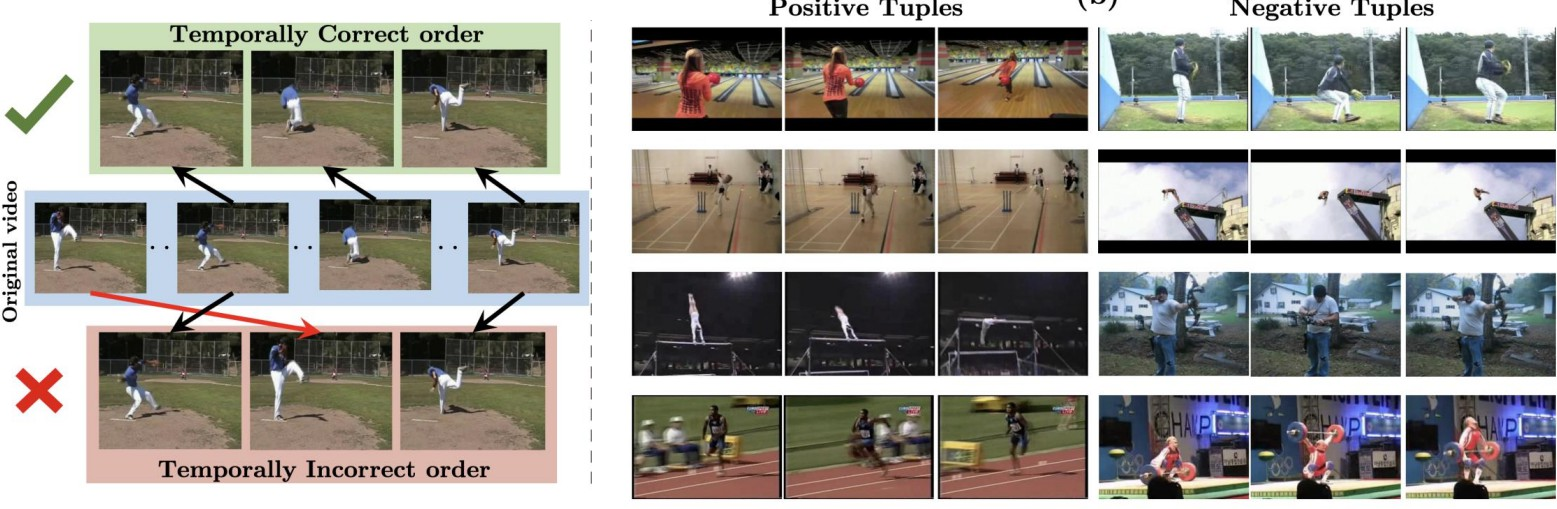
\includegraphics[width=1\textwidth,height=0.6\textheight,keepaspectratio]{images/video/slide_44_1_img.jpg}
    \end{figure}
\framebreak
    \textbf{Objective:} Learn temporal dependencies and motion patterns in videos.
    \begin{itemize}
        \item Given a sequence of video frames, randomly shuffle the order of frames.
        \item The model receives either the original or shuffled sequence.
        \item The objective is to classify whether the input sequence is temporally correct or not.
        \item This encourages the model to learn temporal dependencies and motion patterns in videos.
    \end{itemize}
\framebreak
    \begin{figure}
        \centering
        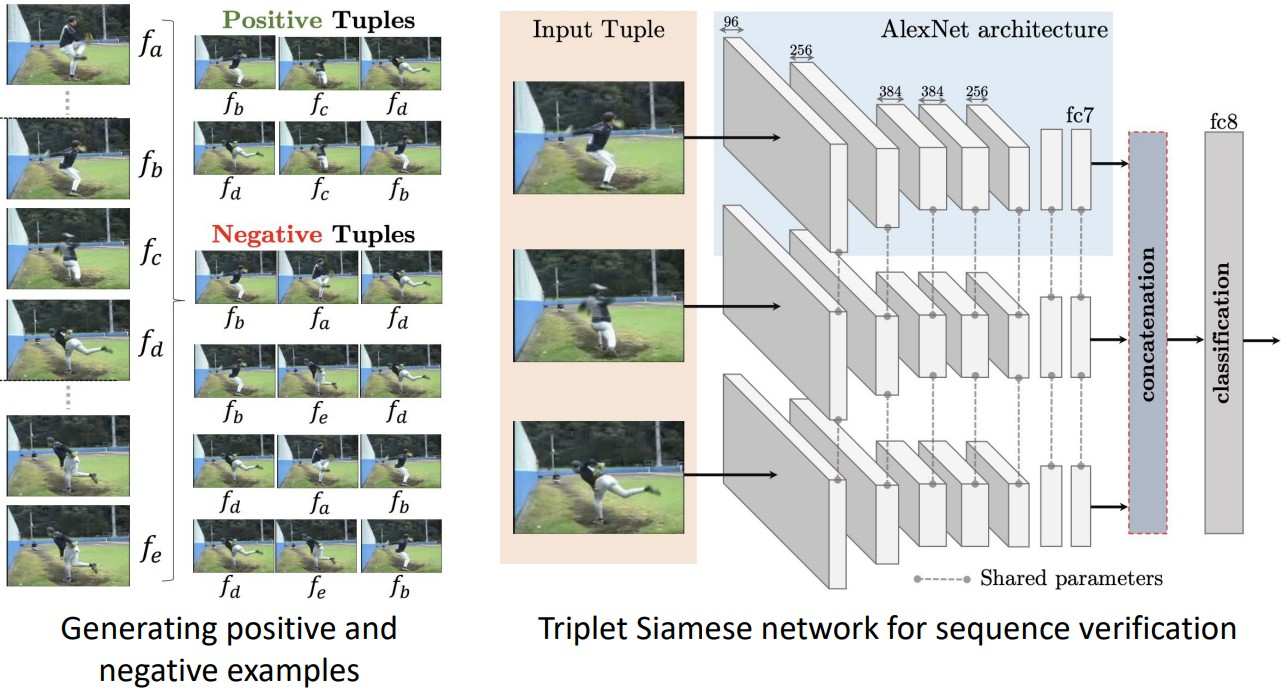
\includegraphics[width=1\textwidth,height=0.9\textheight,keepaspectratio]{images/video/slide_45_1_img.jpg}
    \end{figure}
\framebreak
    \textbf{Transfer Learning:} Fine-tune spatial stream for video classification.
    \begin{figure}
        \centering
        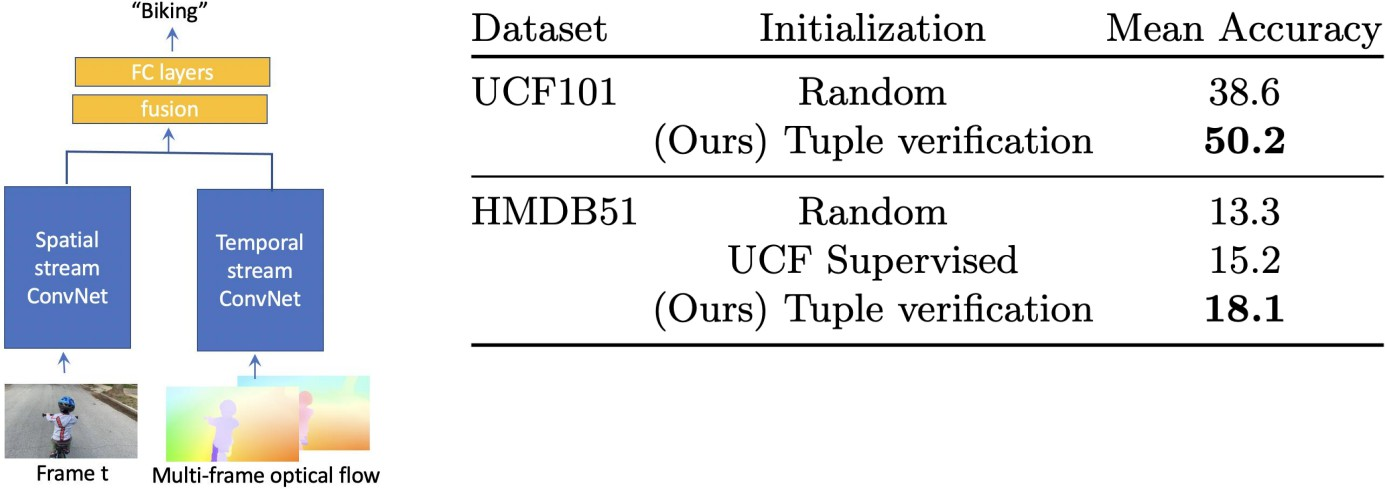
\includegraphics[width=1.07\textwidth,height=0.8\textheight,keepaspectratio]{images/video/slide_46_1_img.jpg}
    \end{figure}
    \footnotesize{[Misra et. al., Shuffle and Learn: Unsupervised Learning using Temporal Order Verification, ECCV 2016]}
\framebreak
    \textbf{Benefits:}
    \begin{itemize}
        \item No need for labeled data, as the task is self-supervised.
        \item Helps the model learn temporal dynamics and motion patterns in videos.
        \item Can be used as a pre-training step before fine-tuning on specific video tasks.
    \end{itemize}
\end{frame}